\subchapter{Bootloader - U-Boot}{Objectives: Set up serial
  communication, compile and install the U-Boot bootloader, use basic
  U-Boot commands, set up TFTP communication with the development
  workstation.}

As the bootloader is the first piece of software executed by a
hardware platform, the installation procedure of the bootloader is
very specific to the hardware platform. There are usually two cases:

\begin{itemize}

\item The processor offers nothing to ease the installation of the
  bootloader, in which case the JTAG has to be used to initialize
  flash storage and write the bootloader code to flash. Detailed
  knowledge of the hardware is of course required to perform these
  operations.

\item The processor offers a monitor, implemented in ROM, and through
  which access to the memories is made easier.

\end{itemize}

The Beaglebone Black board, which uses an AM335x Sitara processor, falls into
the second category. 

The Sitara processors support a multitude of boot sources, and the boot
source is selected by configuring a set of pins at reset.
The Beaglebone limits the choices to one of two options.

The monitor integrated in the ROM reads the internal
eMMC flash chip to search for a valid bootloader.
If the user button is pressed at reset, the Sitara processor will instead search
for a micro-SD card inserted in the connector.

The U-Boot bootloader programmed into the Beaglebone Black boots linux
by executing the contents of the "bootcmd" environment variable, 
which normally is set to use the SD-Card contents, so normally
the button does not have to be pressed.

Therefore, by using an MMC/SD card, we can
start up a Sitara-based board without having anything installed on it.



\section{Setup}

Go to the \code{~/felabs/sysdev/bootloader} directory. 

\section{MMC/SD card setup}

The ROM monitor can read files from a FAT filesystem on the MMC/SD
card. However, the MMC/SD card must be carefully partitionned, and the
filesystem carefully created in order to be recognized by the ROM
monitor. Here are special instructions to format an MMC/SD card
for the Sitara-based platforms.

First, clean out your system log buffer by \code{sudo dmesg -c}, then
connect your card reader to your workstation, with the MMC/SD
card inside. Type the \code{dmesg} command to see which device is used
by your workstation. In case the device is \code{/dev/sdb}, you will see
something like:

\begin{verbatim}
sd 3:0:0:0: [sdb] 3842048 512-byte hardware sectors: (1.96 GB/1.83 GiB)
\end{verbatim}

If your PC has an internal MMC/SD card reader, the device may also been
seen as \code{/dev/mmcblk0}, and the first partition as
\code{mmcblk0p1}. \footnote{This is not always the case with internal
MMC/SD card readers. On some PCs, such devices are behind an internal
USB bus, and thus are visible in the same way external card readers
are}. You will see that the MMC/SD card is seen in the same
way by the IGEPv2 board.

In the following instructions, we will assume that your MMC/SD card
is seen as \code{/dev/sdb} by your PC workstation.

\fbox{\begin{minipage}{\textwidth}
{\bfseries
Caution: read this carefully before proceeding. You could destroy
existing partitions on your PC!

Do not make the confusion between the device that is used by your
board to represent your MMC/SD disk (probably \code{/dev/sda}), and the device
that your workstation uses when the card reader is inserted (probably
\code{/dev/sdb}).

So, don't use the \code{/dev/sda} device to reflash your MMC disk from
your workstation. People have already destroyed their Windows
partition by making this mistake.}
\end{minipage}}

You can also run \code{cat /proc/partitions} to list all block devices
in your system. Again, make sure to distinguish the SD/MMC card from the
hard drive of your development workstation!

Type the \code{mount} command to check your currently mounted
partitions. If MMC/SD partitions are mounted, unmount them:

\begin{verbatim}
$ sudo umount /dev/sdb1
$ sudo umount /dev/sdb2
...
\end{verbatim}

Now, clear possible MMC/SD card contents remaining from previous training 
sessions:

\begin{verbatim}
$ sudo dd if=/dev/zero of=/dev/sdb bs=1M count=256
\end{verbatim}

As we explained earlier, the TI Sitara ROM monitor needs special partition geometry settings
to read partition contents. The MMC/SD card must have 255 heads and 63 sectors.

Let's use the \code{cfdisk} command to create a first partition with these settings:

\code{sudo cfdisk -h 255 -s 63 /dev/sdb}

In the \code{cfdisk} interface, create a first primary partition, starting from the beginning,
with a 512 MB size, a \code{Bootable} type and a \code{0C} type (\code{W95 FAT32 (LBA)}).

You might as well create a partition for the rootfs while you are at it.
Create a new primary partition, starting at the beginning, with 2048 MB size and a \code{83} 
type (\code{Linux})  This code is the default.

Press \code{Write} when you are done.

If you used \code{fdisk} before, you should find \code{cfdisk} much more convenient!

Format the first partition to FAT32, with the \code{boot} label (name):

\begin{verbatim}
sudo mkfs.vfat -n BOOT -F 32 /dev/sdb1
\end{verbatim}

Then format the second partition to \code{EXT4}.

\begin{verbatim}
sudo mkfs -t ext4 -L rootfs /dev/sdb1
\end{verbatim}

Then, remove and insert your card again.

Your MMC/SD card is ready to use.

\section{U-Boot setup}

Download U-Boot from the mainline igep download site:

\begin{verbatim}
wget ftp://ftp.denx.de/pub/u-boot/u-boot-2013.10.tar.bz2
tar xvf u-boot-2013.10.tar.bz2
cd u-boot-2013.10
\end{verbatim}

We want to figure out what is going on, so we will init a git repo.

\begin{verbatim}
git init
git add .
git commit -m "Initial Commit"
\end{verbatim}

Then, apply the
\code{0001-arm-omap-i2c-don-t-zero-cnt-in-i2c_write.patch} patch from
this lab's \code{data} directory:

{\small
\begin{verbatim}
cat /path/to/0001-arm-omap-i2c-don-t-zero-cnt-in-i2c_write.patch | \
   patch -p1
\end{verbatim}
}

or

{\small
\begin{verbatim}
git am /path/to/0001-arm-omap-i2c-don-t-zero-cnt-in-i2c_write.patch
\end{verbatim}
}


Get an understanding of its configuration and compilation steps by
reading the \code{README} file, and specifically the {\em Building the
  software} section.

Basically, you need to:

\begin{itemize}
\item set up the cross compiler 
\begin{verbatim}
export GCCROOT=/usr/local/xtools/arm-unknown-linux-uclibcgnueabi
export PATH=${GCCROOT}/bin:$PATH
export CROSS_COMPILE=arm-linux-
\end{verbatim}

\item Configure U-Boot to build for the Beaglebone Black
\begin{verbatim}
make am335x_boneblack_config
\end{verbatim}

  Note that for our platform, the configuration file is
\begin{verbatim}
include/configs/am335x_evm.h
\end{verbatim}
Read this file to get an
  idea of how a U-Boot configuration file is written;

\item Finally, run \code{make}\footnote{You can speed up the compiling
  by using the \code{-jX} option with \code{make}, where X is the number of parallel
  jobs used for compiling. Twice the number of CPU cores is a good
  value.}, which should build U-Boot.

\end{itemize}

You can now copy the generated \code{MLO} and \code{u-boot.img} files
to the MMC card. \code{MLO} is the first stage bootloader,
\code{u-boot.img} is the second stage bootloader.

You should also create a file \code{uEnv.txt} with the following contents for use in future labs.
Note that the IP address range must not be in use in the training lab. If it is, select another
range like 192.168.1.x.

\begin{verbatim}
ipaddr=192.168.0.100
serverip=192.168.0.1
\end{verbatim}

Copy it to the FAT partition.


Run \code{sudo sync} to make sure it is properly copied

Unmount the MMC card partition.

\section{Setting up serial communication with the board}

Plug the Beaglebone Black board on your computer using the provided
USB-to-serial cable. When plugged-in, a serial port should appear,
\code{/dev/ttyUSB0}.

You can also see this device appear by looking at the output of
\code{dmesg}.

To communicate with the board through the serial port, install a
serial communication program, such as \code{picocom}:

\begin{verbatim}
sudo apt-get install picocom
\end{verbatim}

You also need to make your user belong to the \code{dialout} group to be
allowed to write to the serial console:

\begin{verbatim}
sudo adduser $USER dialout
\end{verbatim}

You need to log out and in again for the group change to be effective.

Run \code{picocom -b 115200 /dev/ttyUSB0}, to start serial
communication on \code{/dev/ttyUSB0}, with a baudrate of 115200. If
you wish to exit \code{picocom}, press \code{[Ctrl][a]} followed by
\code{[Ctrl][x]}.

\section{Testing U-Boot on the MMC card}

Insert the MMC card into the Beaglebone Black board, reset the board while pressing
the "user" button "and check that it boots your new bootloader. You can verify this by checking
the build date: (Should obviously be todays date)

\begin{verbatim}
U-Boot SPL 2013.10-gbd39439-dirty (Mar 03 2014 - 18:03:52)
spl: error reading image args, err - 0
reading u-boot.img
reading u-boot.img


U-Boot 2013.10-gbd39439-dirty (Mar 03 2014 - 20:04:45)

I2C:   ready
DRAM:  512 MiB
WARNING: Caches not enabled
MMC:   OMAP SD/MMC: 0, OMAP SD/MMC: 1
Using default environment

Net:   <ethaddr> not set. Validating first E-fuse MAC
cpsw, usb_ether
Hit any key to stop autoboot:  0 
\end{verbatim}

The message \code{reading u-boot.img} also confirms that U-Boot has
been loaded from the MMC device. The error message is due to the \code{Falcon mode} which
will allow booting the kernel directly from \code{MLO} without loading U-Boot. We do not use this mode.

Interrupt the countdown to enter the U-Boot shell:
\begin{verbatim}
U-Boot #
\end{verbatim}

In U-Boot, type the \code{help} command, and explore the few commands available.
\clearpage
\section{U-Boot Environment}
U-Boot supports an environment, and you can extend the commandset by defining environment variables.
These can be "used" as scripts through the \code{run} command
It is possible to define a compile time environment, which can be extended at run time.
On the Beaglebone Black, the environment can be updated from the file uEnv.txt stored
together with \code{MLO} and \code{u-boot.img} on the SD-Card.

All environment variables are normally displayed in alphabetical order, when printed.
To make it easier to understand, they are displayed in an easier format below.

\begin{lstlisting}
arch=arm
baudrate=115200
board=am335x
board_name=A335BNLT
board_rev=0A5C
boot_fdt=try
bootdelay=1
bootdir=/boot
bootenv=uEnv.txt
bootfile=zImage
bootpart=1:2
console=ttyO0,115200n8
cpu=armv7
ethact=cpsw
ethaddr=c8:a0:30:c4:4e:8f
fdt_high=0xffffffff
fdtaddr=0x80F80000
fdtfile=am335x-boneblack.dtb
filesize=4e
loadaddr=0x80200000
mmcdev=1
mmcroot=/dev/mmcblk0p2 ro
mmcrootfstype=ext4 rootwait
nfsopts=nolock
optargs=quiet drm.debug=7
ramroot=/dev/ram0 rw ramdisk_size=65536 initrd=${rdaddr},64M
ramrootfstype=ext2
rdaddr=0x81000000
rootpath=/export/rootfs
soc=am33xx
spibusno=0
spiimgsize=0x362000
spiroot=/dev/mtdblock4 rw
spirootfstype=jffs2
spisrcaddr=0xe0000
static_ip=${ipaddr}:${serverip}:${gatewayip}:${netmask}:${hostname}::off
stderr=serial
stdin=serial
stdout=serial
usbnet_devaddr=c8:a0:30:c4:4e:8f
vendor=ti
ver=U-Boot 2013.10-gbd39439-dirty (Mar 03 2014 - 20:04:45)
\end{lstlisting}

\clearpage

The most important environment variable is the \code{bootcmd} script which is used to boot linux.

The Beaglebone Black will try to run mmcboot first on the SD-Card, then on the internal eMMC
and finally it will try nandboot (which does not work, since the board does not have a NAND flash)

\begin{lstlisting}
bootcmd=
	run findfdt; 
	run mmcboot;
	setenv mmcdev 1; 
	setenv bootpart 1:2; 
	run mmcboot;
	run nandboot;
		
findfdt=
	if test $board_name = A335BONE; then
		setenv fdtfile am335x-bone.dtb;
	fi;
	if test $board_name = A335BNLT; then
		setenv fdtfile am335x-boneblack.dtb;
	fi;
	if test $board_name = A33515BB; then
		setenv fdtfile am335x-evm.dtb;
	fi;
	if test $board_name = A335X_SK; then
		setenv fdtfile am335x-evmsk.dtb;
	fi;
	if test $fdtfile = undefined; then
		echo WARNING: Could not determine device tree to use;
	fi;
\end{lstlisting}

\clearpage
The normal way of booting is using the internal eMMC or the SD-Card, and
this function is performed by \code{mmcboot}

\begin{lstlisting}
mmcboot=
	mmc dev ${mmcdev};
	if mmc rescan; then
		echo SD/MMC found on device ${mmcdev};
		if run loadbootenv; then
			echo Loaded environment from ${bootenv};
			run importbootenv;
		fi;
		if test -n $uenvcmd; then 
			echo Running uenvcmd ...;
			run uenvcmd;
		fi;
		if run loadimage; then
			run mmcloados;
		fi;
	fi;

loadramdisk=load mmc ${mmcdev} ${rdaddr} ramdisk.gz

loadbootenv=load mmc ${mmcdev} ${loadaddr} ${bootenv}

importbootenv=
	echo Importing environment from mmc ...; 
	env import -t $loadaddr $filesize

loadimage=load mmc ${bootpart} ${loadaddr} ${bootdir}/${bootfile}
\end{lstlisting}

The \code{mmcboot} code will first select the correct MMC device according to \code{mmcdev}.
The MMC device will be initialized through the \code{mmc rescan} command.
If the device is found, then the file \code{uEnv.txt} will be loaded and the contents
will be overlay the current environment, so any environment variable can be 
changed by redefining it in the uEnv.txt file.

If you want to change the boot mechanism, then set the \code{envcmd} variable,
because this will be executed, if it exists.
A typical use was to change the kernel from uImage to zImage.

The environment tries to load the kernel from the root file system
in the \code{/boot} directory, so the rootfs must contain the kernel.

Finally, the the kernel will be booted, using a device tree file.
This is explained on the next page.

\clearpage

If the kernel requires a device tree file (which it does for the Beaglebone Black)
then this is loaded from the \code{/boot} directory.

The Beaglebone Black is using the \code{am335x−-boneblack.dtb} file.

\code{bootz} is used to boot a zImage

\begin{lstlisting}

mmcargs=setenv bootargs console=${console} ${optargs} root=${mmcroot} rootfstype=${mmcrootfstype}

loadfdt=load mmc ${bootpart} ${fdtaddr} ${bootdir}/${fdtfile}

mmcloados=
	run mmcargs;
	if test ${boot_fdt} = yes || test ${boot_fdt} = try; then 
		if run loadfdt; then 
			bootz ${loadaddr} - ${fdtaddr}; 
		else 
			if test ${boot_fdt} = try; then 
				bootz; 
			else
				echo WARN: Cannot load the DT; 
			fi; 
		fi; 
	else 
		bootz; 
	fi;
\end{lstlisting}

NFS Booting can be of interest, and this is supported by the Beaglebone default environment
An easy way to boot from the network, is to set the \code{uenvcmd} variable to \code{run netboot}

\begin{lstlisting}
netargs=setenv bootargs console=${console} ${optargs} root=/dev/nfs nfsroot=${serverip}:${rootpath},${nfsopts} rw ip=dhcp

netboot=
	echo Booting from network ...;
	setenv autoload no; 
	dhcp; 
	tftp ${loadaddr} ${bootfile}; 
	tftp ${fdtaddr} ${fdtfile}; 
	run netargs; 
	bootz ${loadaddr} - ${fdtaddr}
\end{lstlisting}

\clearpage

Finally, the environment supports DFU (Device Firmware Upgrade), SPI Boot and Booting a RAMdisk,
but this is not used on the Beagleboard Black.

\begin{lstlisting}
dfu_alt_info_emmc=rawemmc mmc 0 3751936
dfu_alt_info_mmc=
	boot part 0 1;
	rootfs part 0 2;
	MLO fat 0 1;
	MLO.raw mmc 100 100;
	u-boot.img.raw mmc 300 400;
	spl-os-args.raw mmc 80 80;
	spl-os-image.raw mmc 900 2000;
	spl-os-args fat 0 1;
	spl-os-image fat 0 1;
	u-boot.img fat 0 1;
	uEnv.txt fat 0 1
dfu_alt_info_ram=
	kernel ram 0x80200000 0xD80000;
	fdt ram 0x80F80000 0x80000;
	ramdisk ram 0x81000000 0x4000000

ramargs=setenv bootargs console=${console} ${optargs} root=${ramroot} rootfstype=${ramrootfstype}
ramboot=
	echo Booting from ramdisk ...; 
	run ramargs; 
	bootz ${loadaddr} ${rdaddr} ${fdtaddr}

spiargs=setenv bootargs console=${console} ${optargs} root=${spiroot} rootfstype=${spirootfstype}
spiboot=
	echo Booting from spi ...;
	run spiargs; 
	sf probe ${spibusno}:0; 
	sf read ${loadaddr} ${spisrcaddr} ${spiimgsize}; 
	bootz ${loadaddr}
\end{lstlisting}


\clearpage


\section{Reflashing from U-boot (Skip)}

Since the Beaglebone Black does not have any NAND Flash, the following
chapter is for reference only.

We will flash U-boot and later the kernel and filesystem in NAND
flash. As far as bootloaders are concerned, the layout of the NAND
flash will look like:

\begin{center}
  \includegraphics[width=\textwidth]{labs/sysdev-u-boot/flash-map.pdf}
\end{center}

\begin{itemize}
\item Offset \code{0x0} for the first stage bootloader is dictated by
  the hardware: the ROM code of the OMAP looks for a bootloader at
  offset \code{0x0} in the NAND flash.
\item Offset \code{0x80000} for the second stage bootloader is decided
  by the first stage bootloader. This can be changed by changing the
  U-Boot configuration.
\item Offset \code{0x260000} of the U-Boot environment is also decided
  by the U-Boot configuration.
\end{itemize}

Let's first erase the whole NAND storage to remove its existing
contents. This way, we are sure that what we find in NAND comes from
our own manipulations:

\begin{verbatim}
nand erase.chip
\end{verbatim}

We are going to flash the first stage bootloader in NAND. To do so,
type the following commands:

\begin{verbatim}
mmc rescan
\end{verbatim}

This initializes the MMC interface.

\begin{verbatim}
fatload mmc 0 80000000 MLO
\end{verbatim}
This loads the file from MMC 0 partition 0 to memory at address
0x80000000.

\begin{verbatim}
nandecc hw
\end{verbatim}

This tells U-Boot to write data to NAND using the hardware ECC
algorithm, which the ROM code of the OMAP uses to load the first stage
bootloader.

\begin{verbatim}
nand erase 0 80000
\end{verbatim}

This command erases a 0x80000 byte long space of NAND flash from
offset 0\footnote{Of course, this is not needed here if you erased the
  whole NAND contents as instructed earlier. However, we prefer to
  write it here so that you don't forget next time you write anything
  to NAND.}.

\begin{verbatim}
nand write 80000000 0 80000
\end{verbatim}

This command writes data to NAND flash. The source is 0x80000000
(where we've loaded the file to store in the flash) and the
destination is offset 0 of NAND flash. The length of the copy is
0x80000 bytes, which corresponds to the space we've just erased
before. It is important to erase the flash space before trying to
write on it.

Now that the first stage has been transfered to NAND flash, you can
now do the same with U-Boot.

The storage offset of U-Boot in the NAND is 0x80000 (just after the
space reserved for the first stage bootloader) and the length is
0x1e0000.

After flashing the U-Boot image, also erase the U-boot environment
variables defined by the manufacturer or by previous users of your
board:

\begin{verbatim}
nand erase 260000 80000
\end{verbatim}

You can remove MMC card, then reset the IGEP board. You should see the
freshly flashed U-Boot starting.

You should now see the U-Boot prompt:

\begin{verbatim}
U-Boot #
\end{verbatim}

\clearpage

\section{Setting up Ethernet communication}

Later on, we will transfer files from the development workstation to
the board using the TFTP protocol, which works on top of an Ethernet
connection.

To start with, install and configure a TFTP server on your development
workstation, as detailed in the bootloader slides.

With a network cable, connect the Ethernet port of your board to the
one of your computer. If your computer already has a wired connection
to the network, your instructor will provide you with a USB Ethernet
adapter. A new network interface, probably \code{eth1} or \code{eth2},
should appear on your Linux system.

To configure this network interface on the workstation side, click on
the {\em Network Manager} tasklet on your desktop, and select {\em
  Edit Connections}.

\begin{center}
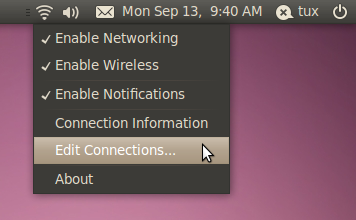
\includegraphics[width=8cm]{labs/sysdev-u-boot/network-config-1.png}
\end{center}

Select the new {\em wired network connection}:

\begin{center}
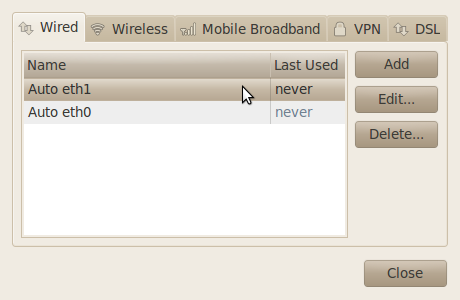
\includegraphics[width=8cm]{labs/sysdev-u-boot/network-config-2.png}
\end{center}

In the \code{IPv4 Settings} tab, press the \code{Add} button
and make the interface use a static IP
address, like \code{192.168.0.1} (of course, make sure that this
address belongs to a separate network segment from the one of the main
company network).

\begin{center}
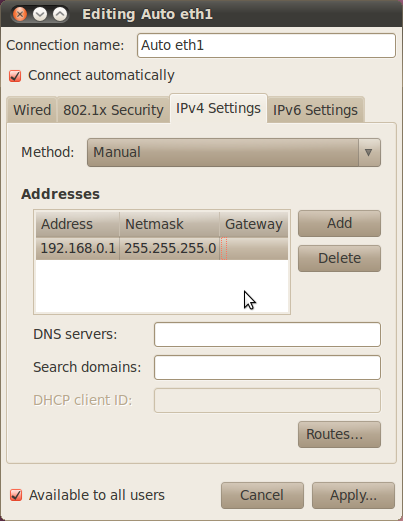
\includegraphics[width=8cm]{labs/sysdev-u-boot/network-config-3.png}
\end{center}

You can use \code{255.255.255.0} as \code{Netmask}, and leave the
\code{Gateway} field untouched (if you click on the \code{Gateway} box, you
will have to type a valid IP address, otherwise you won't be apply to
click on the \code{Apply} button).

The board must also be configured, but if you followed the instructions,
the uEnv.txt file should have set the  network parameters.

Check by

\begin{verbatim}
print ipaddr
print serverip
print ethaddr
\end{verbatim}

If they are not set, or not reasonable, configure the network on the board in U-Boot by setting the \code{ipaddr}
and \code{serverip} environment variables:

\begin{verbatim}
setenv ipaddr 192.168.0.100
setenv serverip 192.168.0.1
\end{verbatim}

If the MAC address is not set, you also need to set it in U-boot,
If this is the case, please contact the teacher and you will be allocated
a number XX.

\begin{verbatim}
setenv ethaddr 01:02:03:04:05:XX
\end{verbatim}

In case the board was previously configured in a different way, we
also turn off automatic booting after commands that can be used to
copy a kernel to RAM:

\begin{verbatim}
setenv autostart no
\end{verbatim}

If you had a NAND flash, then you could have saved the environment by

\begin{verbatim}
saveenv
\end{verbatim}

Since we are running from an MMC card, you have to retype this every time you reboot,
or add it to your \code{uEnv.txt}.

Note the difference in syntax.
\begin{lstlisting}
U-Boot:

	setenv <VAR> <VALUE>

uEnv.txt:

	<VAR>=<VALUE>

\end{lstlisting}



Now switch your board off and on again\footnote{Power cycling your
  board is needed to make your \code{ethaddr} permanent, for obscure
  reasons. If you don't, U-boot will complain that \code{ethaddr} is not
  set.}.

You can then test the TFTP connection. First, put a small text file in
the directory exported through TFTP on your development
workstation. Then, from U-Boot, do:

\begin{verbatim}
tftp 0x80000000 textfile.txt
\end{verbatim}

{\bf Caution: known issue in Ubuntu 12.04 and later}:
if this command doesn't work, you may have to stop the server
and start it again every time you boot your workstation:

\begin{verbatim}
sudo service tftpd-hpa restart
\end{verbatim}

The \code{tftp} command should have downloaded
the \code{textfile.txt} file from your development
workstation into the board's memory at location 0x80000000 (this
location is part of the board DRAM). You can verify that the download
was successful by dumping the contents of the memory:

\begin{verbatim}
md 0x80000000
\end{verbatim}

We will see in the next labs how to use U-Boot to download, flash and
boot a kernel.

\section{Rescue binaries}

If you have trouble generating binaries that work properly, or later
make a mistake that causes you to loose your \code{MLO} and
\code{u-boot.img} files, you will find working versions under
\code{data/} in the current lab directory.
